\section{Evaluation}
\label{sec:evaluation}
% Provide an introductory paragraph that summarizes what's in this section: a list of runs/experiments intended to test your implementation and ideas. Describe each of these experiments in a few words/a sentence.
The Evaluation section presents the experimental setup, performance metrics, and analysis of the ray tracing implementation under various conditions. The computational platform and software environment are detailed to provide context for the hardware and tools used. The methodology outlines the procedures for measuring runtime and calculating speedup, while the results focus on the effects of workload distribution strategies and scene complexity on parallel performance. This section concludes with an analysis of memory usage and its impact on scalability.


\subsection{Computational Platform and Software Environment}
\label{subsec:computational-platform-and-software-environment}

\subsubsection{System Overview}
The experiments were conducted on four CPU nodes of the Perlmutter supercomputer at the National Energy Research Scientific Computing Center (NERSC). Each node was running \textit{SUSE Linux Enterprise Server 15 SP4} with kernel version \textit{5.14.21-150400.24.81\_12.0.87-cray\_shasta\_c}. Each node is equipped with two AMD EPYC 7763 (Milan) processors.

\subsubsection{CPU Specifications}
Each AMD EPYC 7763 processor has 64 cores running at a clock rate of 2.45\,GHz and supports Simultaneous Multi-Threading (SMT), allowing two threads per core. Each core is equipped with:
\begin{itemize}
    \item 32\,KiB L1 cache,
    \item 512\,KiB L2 cache,
    \item 32\,MiB L3 cache shared among 8 cores.
\end{itemize}
The processor supports 8 memory channels per socket, with 2 DIMMs per channel, and is configured with 4 NUMA domains per socket (NPS=4). The system is equipped with 256\,GiB of DDR4 DRAM, providing a memory bandwidth of 204.8\,GiB/s per CPU~\cite{nersc_perlmutter_architecture, amd_epyc_tuning_guide}.

\subsubsection{Software Environment}
The code was parallelized using OpenMP 4.5~\cite{openmp_spec}, which provides a portable and scalable model for shared memory parallel programming. The code was compiled using the following flags:
\begin{itemize}
    \item \texttt{-O3}: Enables high-level compiler optimizations.
    \item \texttt{-fopenmp}: Enables OpenMP directives for multi-threading.
\end{itemize}

The experiments utilized the following OpenMP environmental variables:
\begin{itemize}
    \item \texttt{OMP\_SCHEDULE={schedule}}: Specifies the thread scheduling policy.
    \item \texttt{OMP\_NUM\_THREADS={thread counts}}: Configures the number of threads used.
    \item \texttt{OMP\_PLACES=threads}: Maps each OpenMP thread to a separate hardware thread, ensuring efficient resource usage.
    \item \texttt{OMP\_PROC\_BIND=spread}: Distributes threads evenly across the available CPUs for optimal workload balancing.
\end{itemize}

\subsection{Methodology}
\label{subsec:methodology}
% % Describe the procedures you use to test your system.

% % Performance metrics: describe exactly what metrics you employ to measure performance. It might be elapsed time from instrumentation code you added around the main computational code. Later in the term, it may be something else.


We evaluated the performance of various MM methods using matrix sizes of \(128 \times 128\), \(512 \times 512\), and \(2048 \times 2048\). For the Basic and Blocked OpenMP implementations, we tested with thread counts of 1, 4, 16, and 64 to observe the impact of varying concurrency levels on performance.

\subsubsection{Runtime}
\label{subsubsec:runtime}
Runtime was measured using the \textit{high\_resolution\_clock} of the C++ \textit{std::chrono} library. To demonstrate the process, we use simplified pseudo-code in Listing~\ref{listing:measuring-elapsed-time}, which highlights the key steps in measuring the runtime.

\begin{lstlisting}[caption={Simplified pseudo-code for measuring the runtime of ray tracing.},label={listing:measuring-elapsed-time},name=measuring-elapsed-time,float=htbp,style=mystyle,language=C++]
// Before starting the timer, we initialize image, camera and scene.

start_time = now();
#pragma omp parallel for
for each pixel (x, y) in image:
    for each sample in samples_per_pixel:
        r = get_ray(x, y)
        images[x, y] += ray_color(r, max_depth, world)
end_time = now();
runtime = end_time - start_time;

// After stopping the timer, we write image to output file
\end{lstlisting}

\subsubsection{Speedup}
\label{subsubsec:speedup}
Speedup was defined as the ratio of a parallel program's execution time compared to a sequential program's execution time. For a problem size \(n\) and \(p\) parallel threads, the speedup \(S(n, p)\) was calculated as follows:

\begin{displaymath}
    S(n, p) = \frac{T^*(n)}{T(n, p)}
\end{displaymath}

Here, \(T^*(n)\) represents the runtime of the best serial algorithm for a problem of size \(n\). In our case, this was the runtime recorded for \(\texttt{OMP\_NUM\_THREADS=1}\).

\subsection{Workload Distribution Study}
\label{subsec:workload-distribution-study}

The workload distribution study focuses on analyzing the impact of different scheduling strategies on parallel performance. This experiment evaluates the runtime and speedup for static and dynamic scheduling methods across thread counts of 1, 2, 4, 8, 16, 32, 64, 128, and 256. The configurations include static scheduling, dynamic scheduling with a chunk size of 1 (\texttt{dynamic-1}), and dynamic scheduling with a chunk size of 16 (\texttt{dynamic-16}).

For lower thread counts (2, 4, and 8), both \texttt{dynamic-1} and \texttt{dynamic-16} outperform static scheduling, as shown in Figure~\ref{fig:load-imbalance-speedup}. The dynamic approaches provide better load balancing, reducing runtime compared to the static method. However, as the thread count increases beyond 8, the performance of static scheduling converges with that of \texttt{dynamic-1}, with static even slightly outperforming \texttt{dynamic-1} at higher thread counts. This performance crossover is attributed to reduced scheduling overhead in static scheduling when many threads are utilized.

Dynamic scheduling consistently outperforms static scheduling, but the performance gap becomes significant with a thread count of 256. Specifically, \texttt{dynamic-1} achieves a speedup of 21.8 times, compared to 18.9 times for static scheduling. The large disparity is attributable to the limited height of the image (288 pixels), which constrains the number of iterations being parallelized by static scheduling. 

As shown in the \texttt{ray\_color} function in Listing~\ref{listing:ray-color}, simulating the ray color for the sky region is relatively computationally light. When a ray does not intersect any objects in the scene, no recursion is necessary, significantly reducing the computational workload for these regions. Furthermore, as shown in Figure~\ref{fig:sample-image-fine}, the upper part of the image generated in our testing is largely sky without objects, making the static scheduling inefficient due to the uneven workload distribution.

These findings indicate that while dynamic scheduling is effective for addressing load imbalance, the choice of chunk size and the problem size significantly influence performance. Future studies should explore configurations with larger workloads and higher scene complexity to better utilize the available computational resources.

\begin{figure}[htbp]
    \centering
    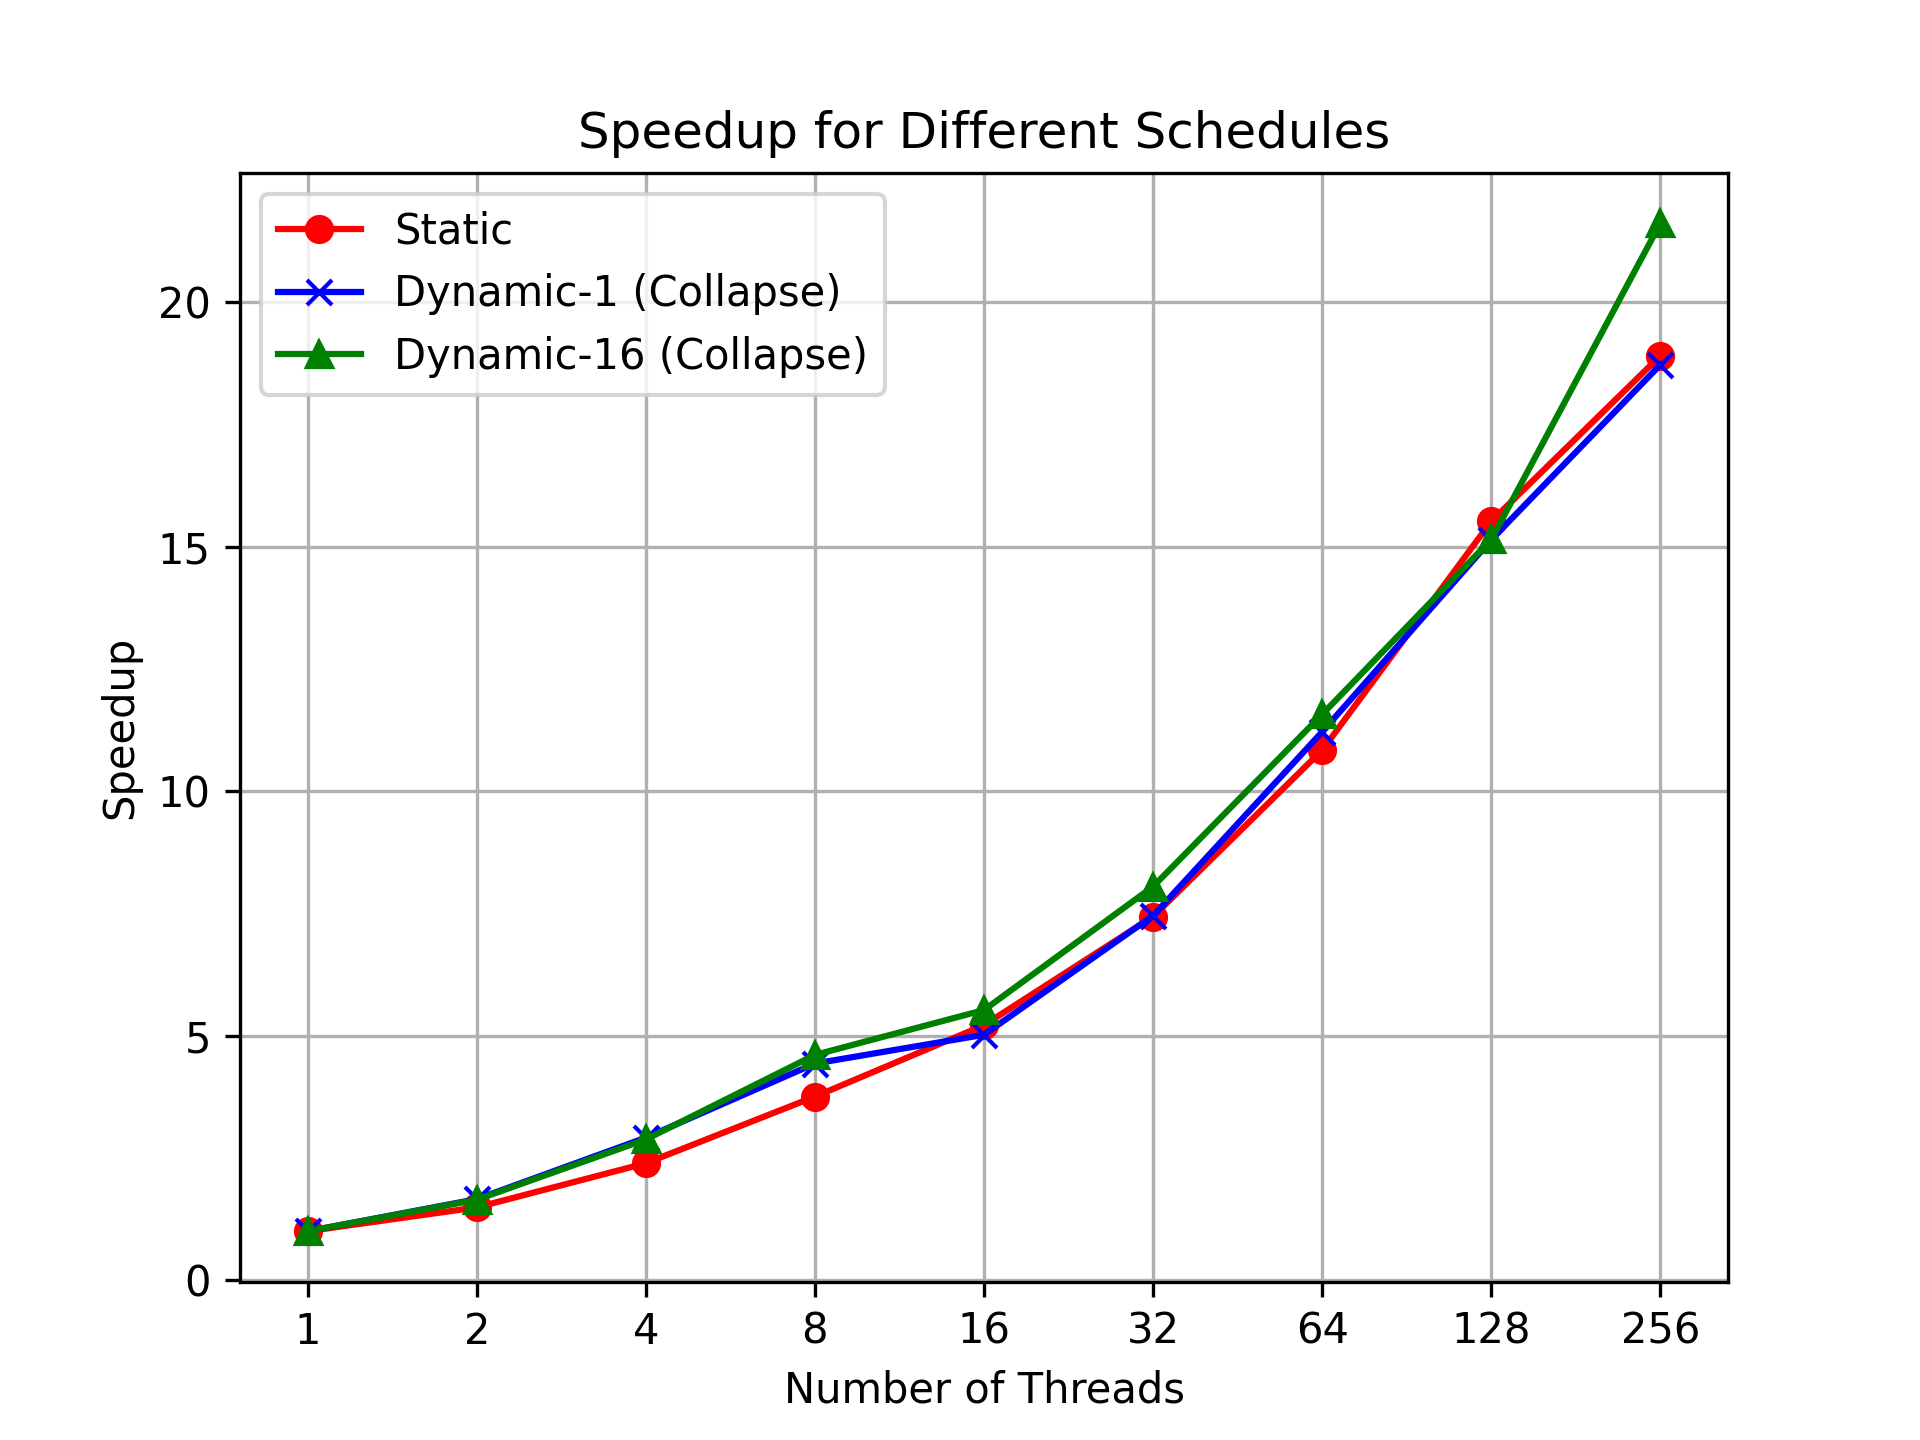
\includegraphics[width=1.0\linewidth]{images/load_imbalance_speedup_comparison.png}
    \caption{Comparison of speedup across different scheduling strategies (static and dynamic) with varying chunk sizes. The results highlight the trade-offs between load balancing and scheduling overhead.}
    \label{fig:load-imbalance-speedup}
\end{figure}

\FloatBarrier
\subsection{Weak Scaling Study}
\label{subsec:weak-scaling-study}

The weak scaling study evaluates the performance of the ray tracing implementation as the problem size, measured by scene complexity, increases. This experiment measures runtime and speedup for scene complexities ranging from 1 to 64 and thread counts of 1, 2, 4, 8, 16, 32, 64, 128, and 256. Dynamic scheduling with a chunk size of 1 was used for all configurations.

The results indicate that more complex scenes benefited significantly from parallelization. For example, at a scene complexity of 1, the maximum speedup achieved was only 1.3 times using 256 threads. In contrast, a scene complexity of 64 achieved a speedup of 77.5 times with 256 threads. This highlights the significant impact of scene complexity on the efficiency of parallel execution. As shown in Figure~\ref{fig:scene-complexity-speedup}, scaling performance improves with increasing scene complexity; however, the performance gains plateau as scene complexity reaches 64.

The performance plateau at higher scene complexities suggests potential bottlenecks such as synchronization overhead, memory contention, or limitations inherent to the computational platform. These findings emphasize the importance of optimizing workload distribution and employing larger problem sizes to better utilize parallel resources. Further investigation is required to determine the exact causes of the performance plateau, which could include analyzing memory access patterns, thread synchronization mechanisms, or identifying architectural constraints. Additional details on memory usage inefficiencies and their impact on scaling behavior are discussed in Appendix~\ref{sec:memory-footprint}.

\begin{figure}
    \centering
    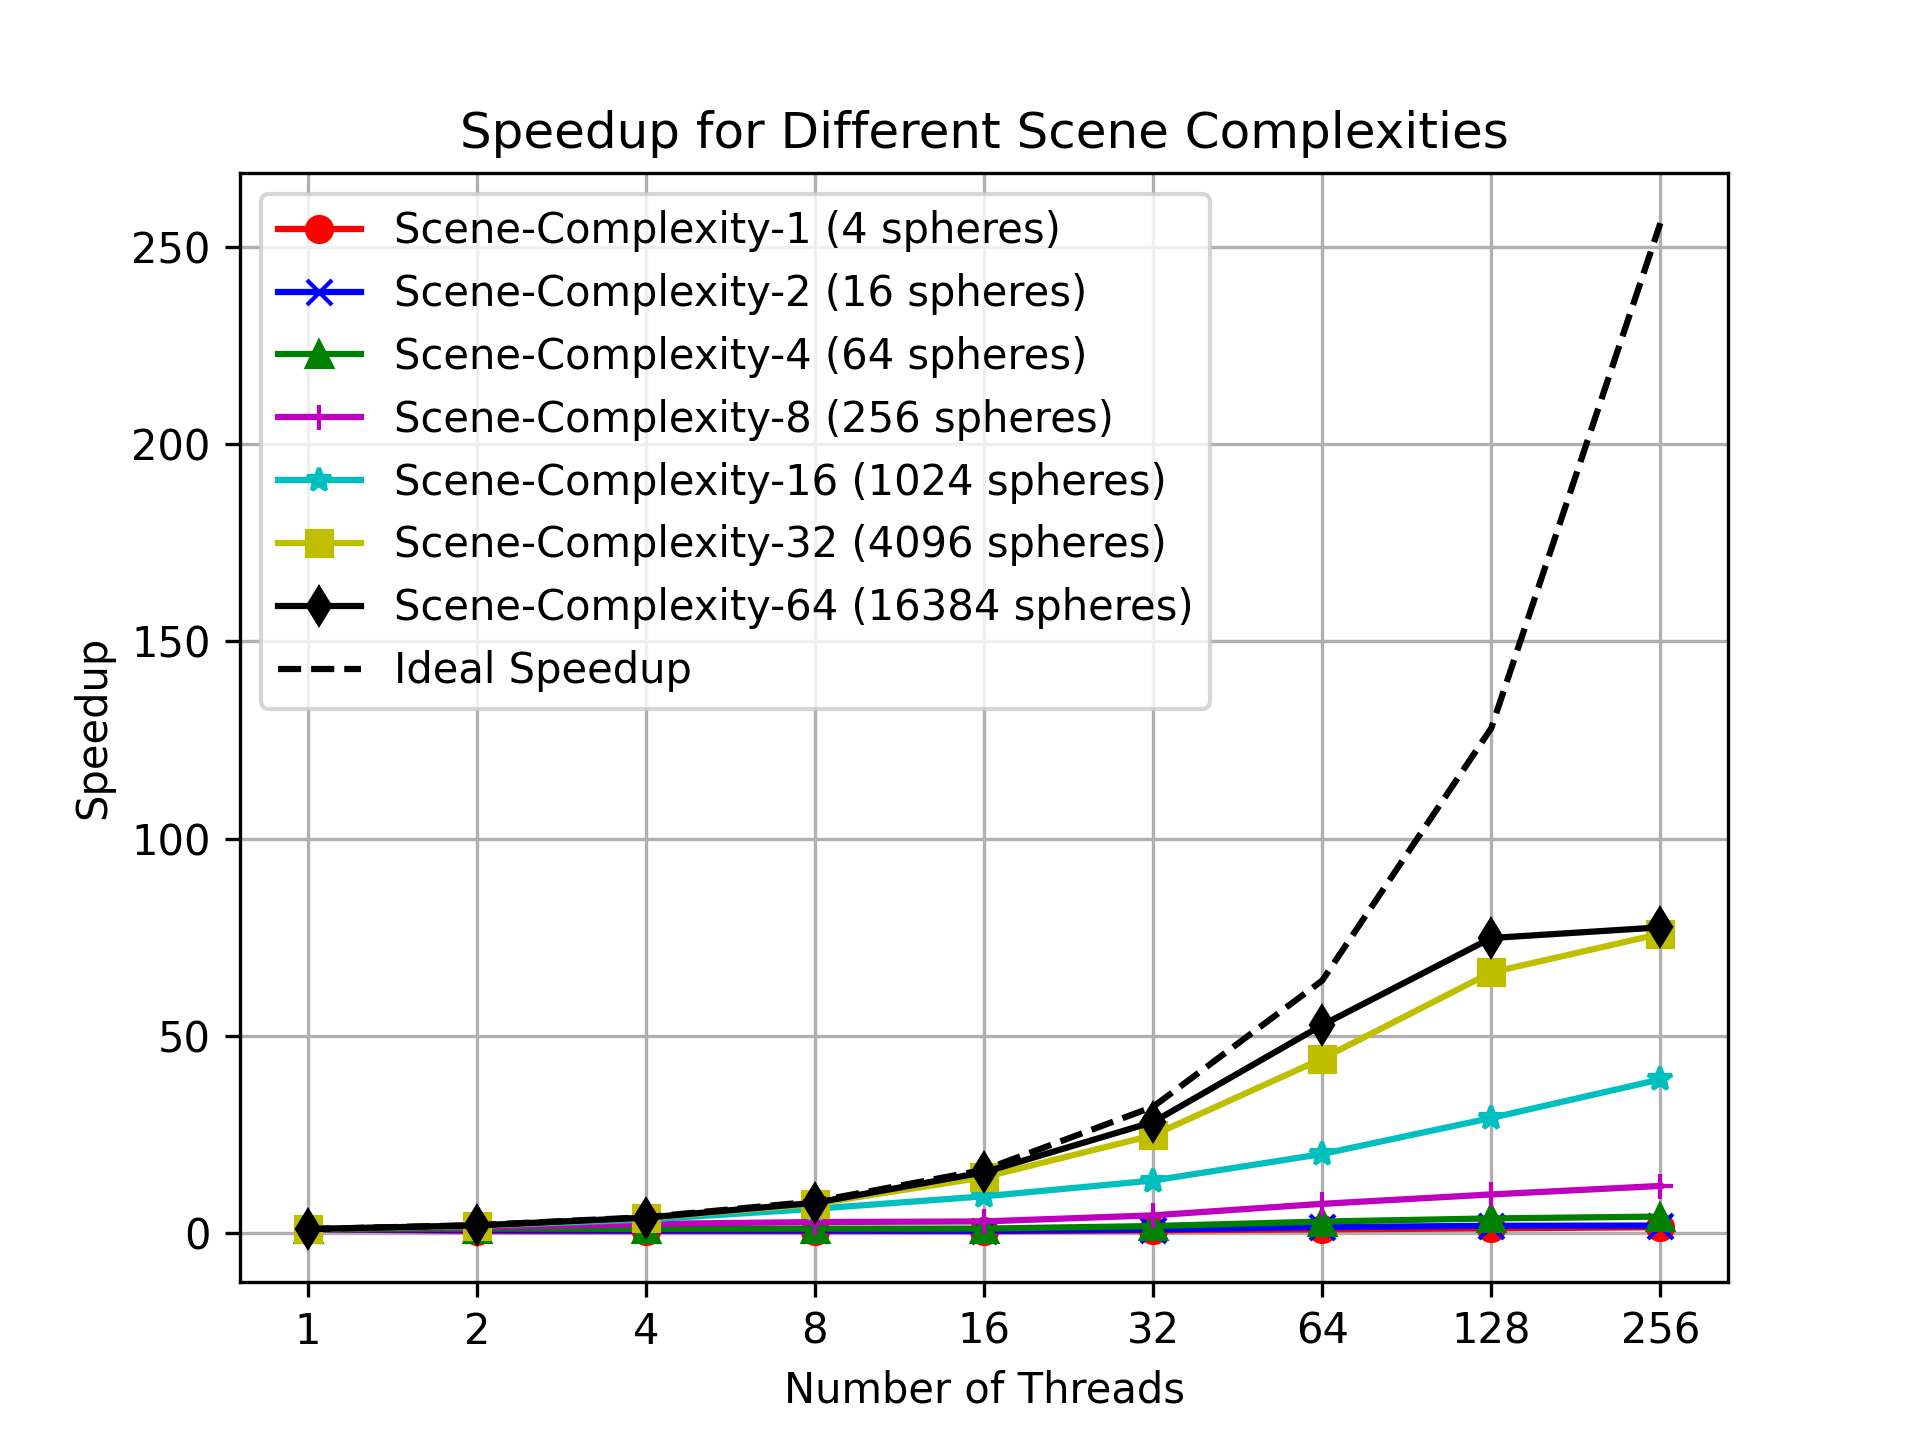
\includegraphics[width=1.0\linewidth]{images/scene_complexity_speedup_comparison.png}
    \caption{Speedup achieved for varying scene complexities under dynamic scheduling. The results demonstrate improved scaling for higher complexities, but with diminishing returns as complexity increases.}
    \label{fig:scene-complexity-speedup}
\end{figure}
\FloatBarrier

\begin{comment}
%% the material that follows is from the generic tech paper skeleton project


How our solution performed, how its performance compared to that of other solutions mentioned in related work, and how these results show that our solution is effective
\begin{itemize}
    \item Presentation and Interpretation
    \item Why, how, and to what degree our solution is better
    \item Why the reader should be impressed with our solution
    \item Comments
    \item Here is a cross reference to Table~\ref{tab:my_label} and Fig.~\ref{fig:my_label}.
\end{itemize}

Context and limitations of our solution as required for summation
\begin{itemize}
    \item What the results do and do not say
\end{itemize}

\end{comment}